% !TEX root = ../MasterThesis_Onoe.tex
% 上記はただのコメントではなく親ファイルの場所を教えているので
% 消してしまうとファイルごとのタイプセットができなくなるので注意。
% 親ファイル名を変更したときはここも変更する。

\chapter{深層学習} \label{sec:Deeplearning}
本章では、本研究で提案する手法である深層学習の理論を述べる。初めに4.1節で深層学習の基礎技術であるパーセプトロンについて説明し、パーセプトロンを多層にしたニューラルネットの構造と計算技術について説明する。そして4.2節で深層学習のネットワークについて、特にグラフ構造のデータを扱うグラフニューラルネットワークについて紹介する。
\section{ニューラルネットワーク}
\subsection{パーセプトロン(単層ニューラルネットワーク)}
ニューラルネットワークの基礎となるパーセプトロンは、ローゼンブラットにより1957年に考案された\cite{perceptron}。パーセプトロンの基本構造は、信号を入力として受け取り論理回路を通して出力信号を出すものである。図\ref{perceptron}に最も基本的なパーセプトロンの例\cite{dnnbook}を示す。
\begin{figure}[H]
	\begin{center}
 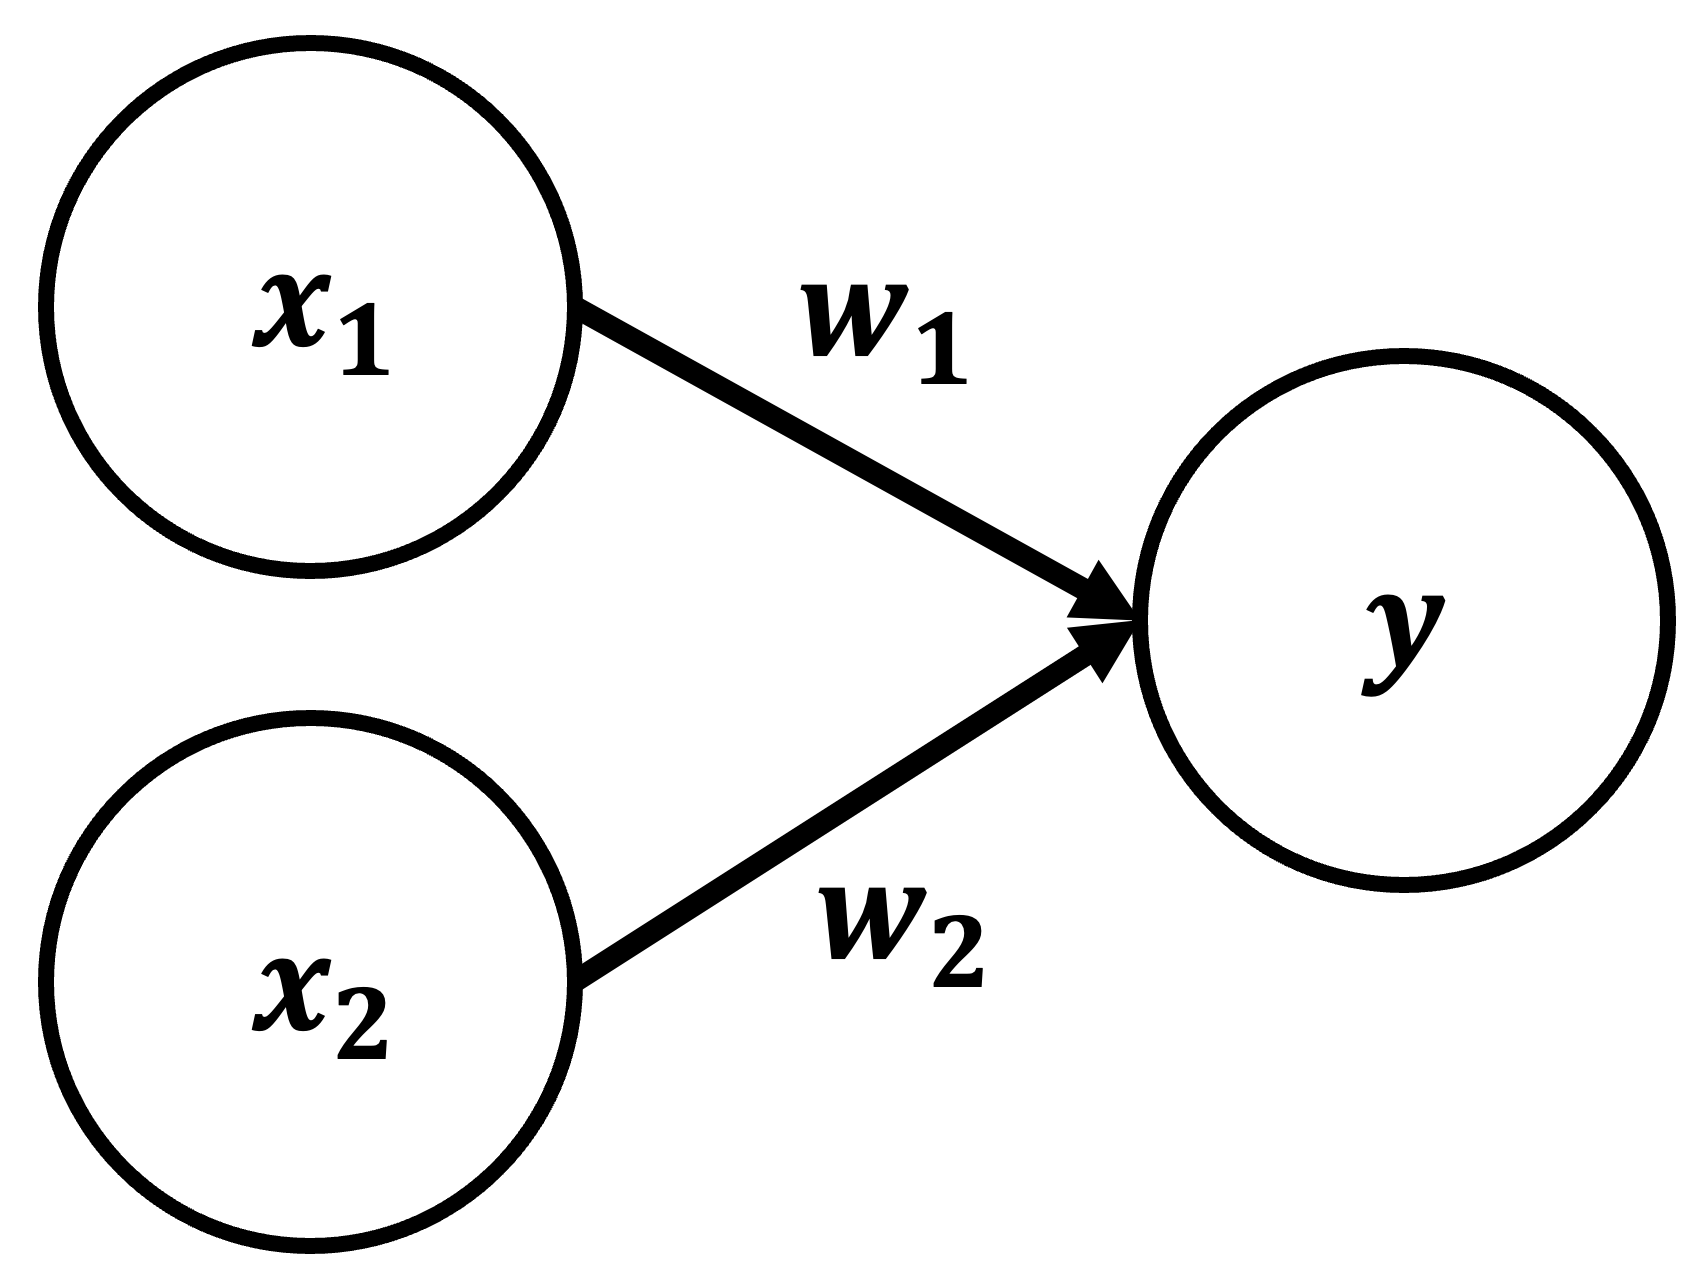
\includegraphics[keepaspectratio, scale=0.15]
 	{Figure/Deeplearning/perceptron.png}
 		\caption{パーセプトロン}
 		\label{perceptron}
	\end{center}
\end{figure}
$x_1, x_2$は入力信号、$y$が出力信号であり、$w_1,w_2$がそれぞれの入力信号にかかる重みを表す。また、図中における$\bigcirc$はノードと呼ぶ。入力信号はノードに送られる前に重みが掛けられ、出力ノードにてそれらの総和をとる。出力ノードでの演算(活性化関数)をステップ関数(階段関数)とすると、その総和が閾値$\theta$を超えている場合のみ出力信号は1を出力することになる。数式で示すと以下のようになる。
\begin{align}
 y =
 \begin{cases}
 0 & (w_1x_1 + w_2x_2 ) \leq \theta\\
 1 & (w_1x_1 + w_2x_2 ) > \theta \\
 \end{cases}
\end{align}

パーセプトロンにおいて重要となるのは入力信号に対する固有の重みであり、重みは各信号の重要性を操作する要素として働く。すなわち重みが大きいほど、対応する信号の全体における重要性が高くなる。この重みを更新する操作を学習と呼び、ニューラルネットワークでは学習を繰り返すことで重みパラメータを理想とする値に近づけていく。

また、入力信号が3つ以上の場合についても考えることができ、以下のような式で表される。入力信号$x = \{ x_1, x_2, \ldots, x_n \}$、重みパラメータ$w = \{ w_1, w_2, \ldots, w_n \}$、活性化関数(ここではステップ関数)を$h(x)$とすると、出力ベクトルyは以下のようになる。
\begin{align}
y = h(w^T x) =
 \begin{cases}
 0 & (w_1x_1 + w_2x_2 + \ldots + w_nx_n) \leq \theta\\
 1 & (w_1x_1 + w_2x_2 + \ldots + w_nx_n) > \theta \\
 \end{cases}
\end{align}
\subsection{多層パーセプトロン(多層ニューラルネットワーク)}
パーセプトロンの演算では線形領域のみしか表現できず、非線形領域においても扱えるよう入力層と出力層の間に中間層(隠れ層)を加えるニューラルネットワークに改良された。このような中間層を複数重ねたパーセプトロンを多層パーセプトロン(Multi Layer Perceptron; MLP)と呼ぶ。多層パーセプトロンの簡単な例を図\ref{mlp}に示す。\\
\begin{figure}[H]
	\begin{center}
 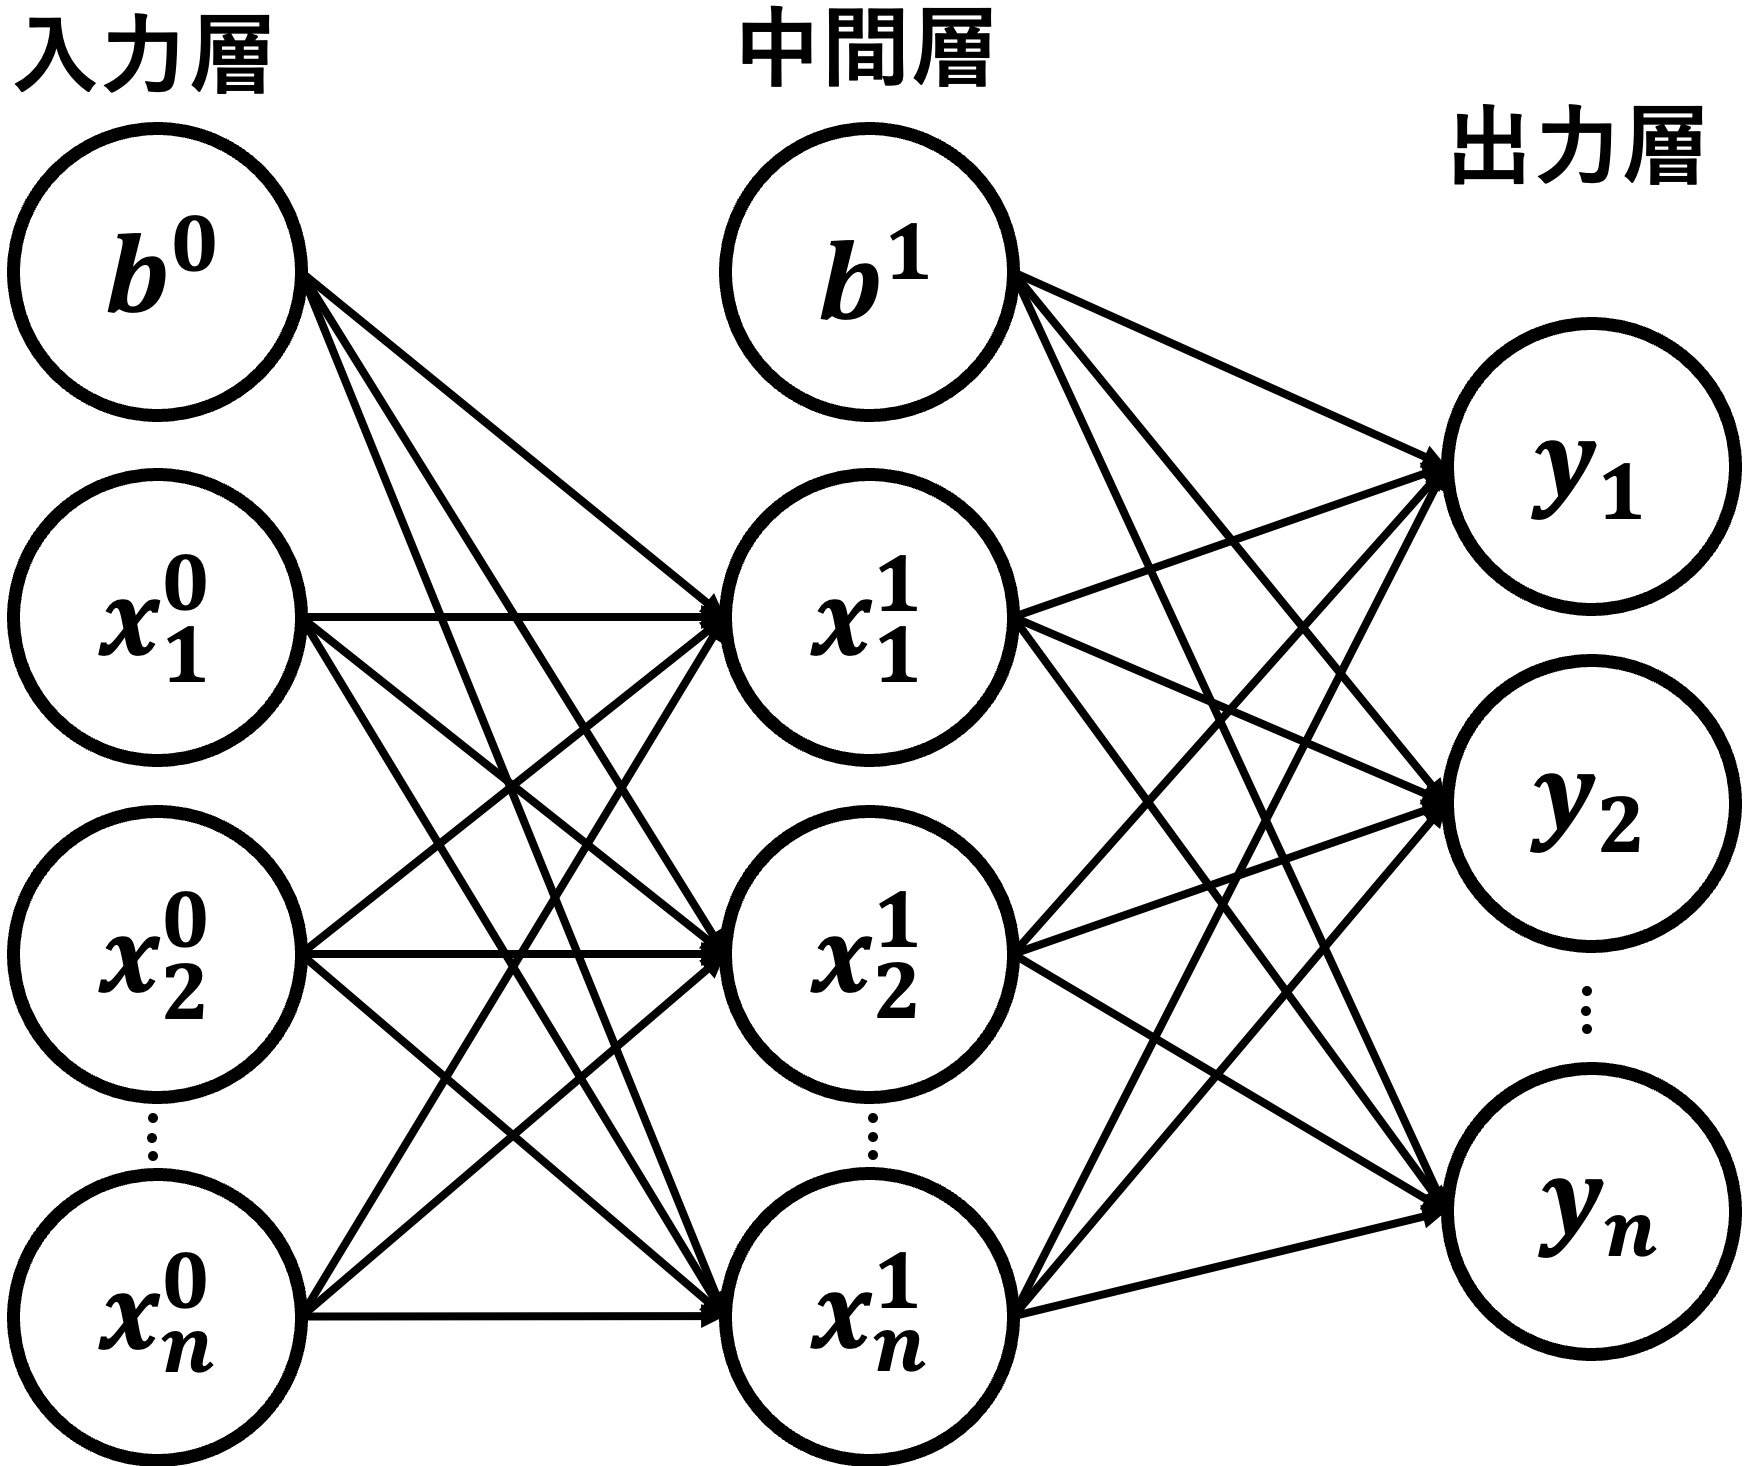
\includegraphics[keepaspectratio, scale=0.2]
 	{Figure/Deeplearning/mlp.png}
 		\caption{多層パーセプトロン(ニューラルネットワーク)}
 		\label{mlp}
	\end{center}
\end{figure}
最も左のノード列を入力層、真ん中のノード列を中間層、一番右のノード列を出力層とすると、以下のような数式で表される。入力信号$x^0 = \{ x_1^0, x_2^0, \ldots, x_n^0 \}$、中間層の各ノードに入ってくる信号$x^1 = \{ x_1^1, x_2^1, \ldots, x_n^1 \}$、入力層と中間層の信号にかかる重みパラメータがそれぞれ$w^0 = \{ w_1^0, w_2^0, \ldots, w_n^0 \}, w^1 = \{ w_1^1, w_2^1, \ldots, w_n^1 \}$、活性化関数を$h(x)$とすると、出力ベクトル$y_n$は
\begin{align}
x_1^1 = h(w_1^0 x_1^0 + w_2^0 x_2^0 + w_3^0 x_3^0 + \cdots + w_n^0 x_n^0 + b^0)\\
y_n = h(w_1^1 x_1^1 + w_2^1 x_2^1 + w_3^1 x_3^1 + \cdots + w_n^1 x_n^1 + b^1)
\end{align}
となる。ここで、$b^n$としてより学習にパラメータを加えるため、各層に実数値のバイアスを導入した。重みと信号の積の和を$a$として、上式に行列を用いると簡略に表現できる。
\begin{align}
\bm{y} = h(\bm{a})\\
\bm{a} = \bm{W} \bm{x} + \bm{b}
\end{align}
 以下ではニューラルネットワークの学習における、学習の仕組みや重要な技術について取り上げる。
\subsubsection{活性化関数}
活性化関数はニューラルネットワークにおける入力の重み線形和から、出力を決定するための関数である。活性化関数には、非線形演算によって多層構造での表現力を高めるために非線形関数が用いられ、以下に主なものについて示しそれぞれの関数のグラフを図\ref{acti}に示す。中でもReLU関数は、勾配の最大値が1であることから勾配消失を起こしにくく、計算の安定性の理由から多くのモデルにおいて用いられている。(sigmoid関数の場合$x=0$で最大となり、それ以外で急速に小さくなってしまう)
\begin{itemize}
	\item ステップ(階段)関数
		\begin{align}
			h(a) =
			\begin{cases}
			0 & (a \leq \theta)\\
			1 & (a > \theta)
			\end{cases}
		\end{align}
	\item sigmoid関数
		\begin{equation}
			h(a) = \frac{1}{1+\exp(-a)}
		\end{equation}
	\item $\tanh$関数
		\begin{equation}
			h(a) = \tanh(a)
	\end{equation}
	\item ReLU関数(ランプ関数)
		\begin{align}
			h(a) =
			\begin{cases}
			0 & (a \leq \theta)\\
			a & (a > \theta)
			\end{cases}
		\end{align}
	\item LeakyReLU関数 (s=0.01が多い)
		\begin{align}
			h(a) =
			\begin{cases}
			sa & (a \leq \theta)\\
			a & (a > \theta)
			\end{cases}
		\end{align}
\end{itemize}
\begin{figure}[H]
  \begin{minipage}[b]{0.45\linewidth}
   \centering
    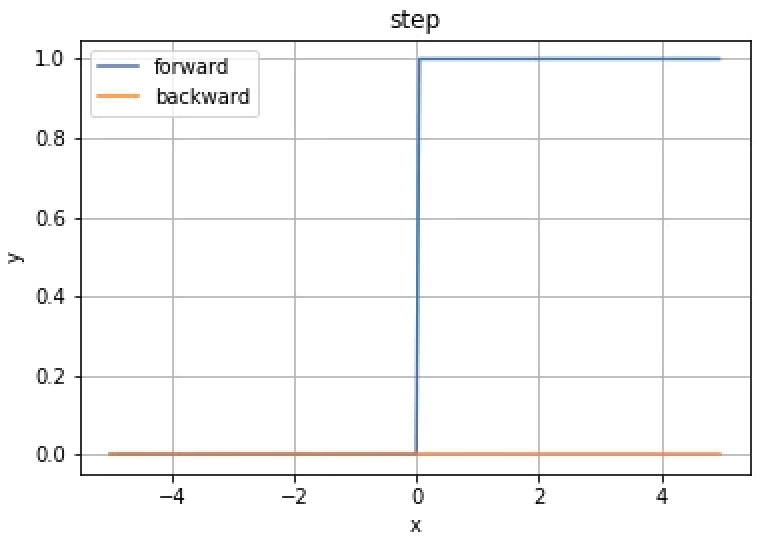
\includegraphics[keepaspectratio, scale=0.25]{Figure/Deeplearning/step.png}
    \subcaption{ステップ関数}
  \end{minipage}
    \begin{minipage}[b]{0.45\linewidth}
    \centering
    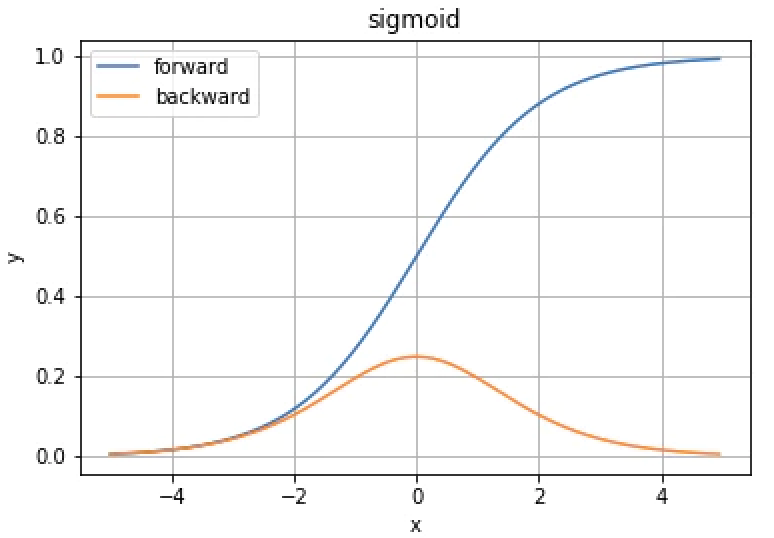
\includegraphics[keepaspectratio, scale=0.25]{Figure/Deeplearning/sigmoid.png}
    \subcaption{sigmoid関数}
  \end{minipage}
  \begin{minipage}[b]{0.45\linewidth}
  \centering
    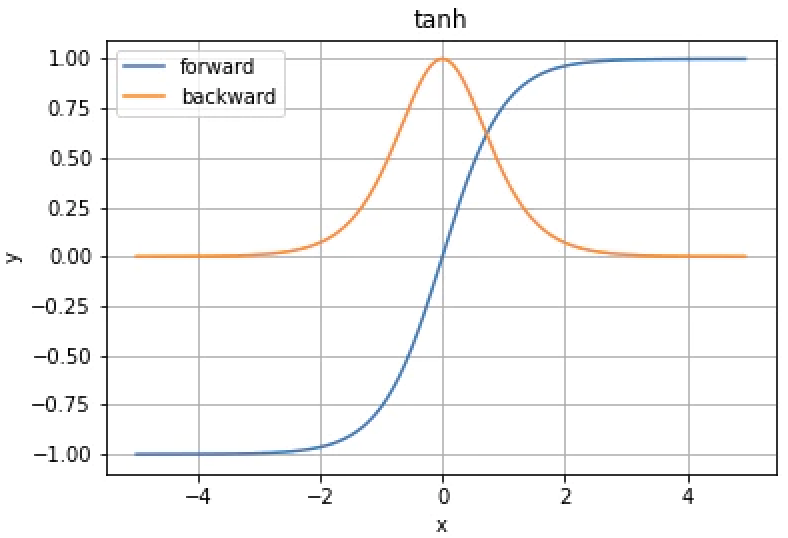
\includegraphics[keepaspectratio, scale=0.25]{Figure/Deeplearning/tanh.png}
    \subcaption{$\tanh$関数}
   \end{minipage}
  \begin{minipage}[b]{0.45\linewidth}
  \centering
    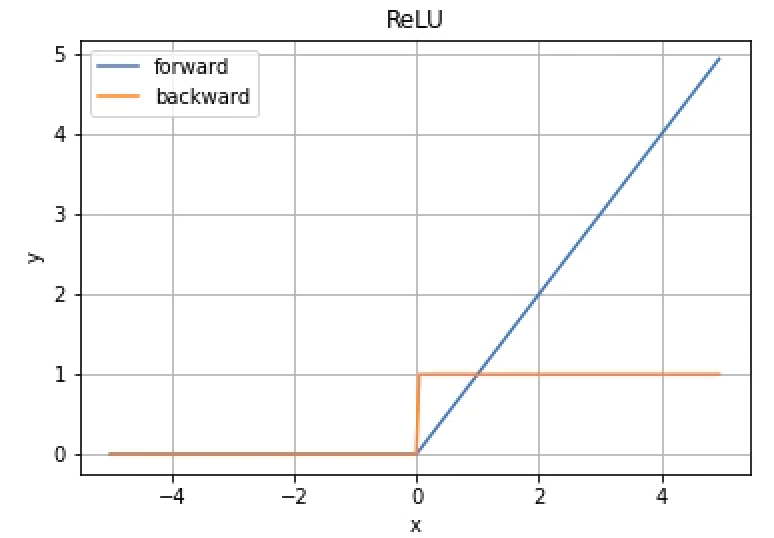
\includegraphics[keepaspectratio, scale=0.25]{Figure/Deeplearning/ReLU.png}
    \subcaption{ReLU関数}
  \end{minipage}
  \begin{minipage}[b]{0.45\linewidth}
  \centering
    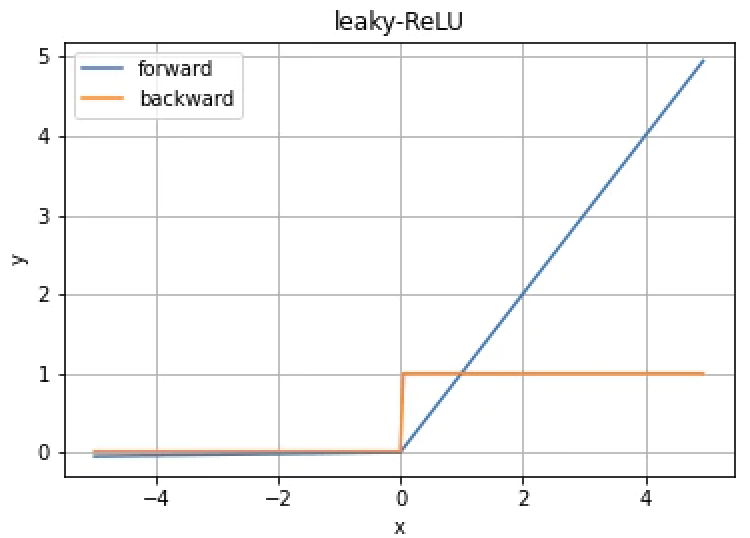
\includegraphics[keepaspectratio, scale=0.25]{Figure/Deeplearning/LeakyReLU.png}
    \subcaption{LeakyReLU関数}
  \end{minipage}
  \caption{活性化関数のグラフ。Forwardは順方向、backwardは逆方向 (後に誤差逆伝播法で説明) の際の演算を表す。}
  \label{acti}
\end{figure}
\subsubsection{出力層の設計}
ニューラルネットワークで扱える問題は、主に回帰問題と分類問題に分けられる。それぞれの問題によって出力層の設計が異なり、回帰問題においては恒等関数が、分類問題においてはソフトマックス関数が用いられる。恒等関数では入力された値をそのまま出力する。ソフトマックス関数は以下の式\ref{softmax}のように、0から1までの値を出力する関数であり、それぞれのカテゴリに分類される確率を表す。ここで$y_k$はニューラルネットワークの出力、$x_k$は出力層へ入ってくる信号を表す。また、出力層のノード数は問題に合わせて適宜調整する必要があり、分類問題であればカテゴリ数だけノードを設計する必要がある。
\begin{align}
\label{softmax}
y_k = \frac{\exp(x_k)}{\sum_{i=1}^n \exp(x_i)}
\end{align}

\subsubsection{損失関数}
先述の通り、ニューラルネットワークでは学習によって重みを更新するが、その際に学習結果を正しい答えと照らし合わせて評価し、その評価値を最小にするように重みを更新する。この評価関数を損失関数 (loss function) と呼ぶ。損失関数には主に以下の2つが用いられる。
\begin{itemize}
	\item 二乗和誤差関数  (Mean Squared Error) \\
		二乗和誤差関数は、以下の式\ref{mse}で定義される関数である。ここで、$y_k$はニューラルネットワークの出力、$t_k$は正解ラベルを表し、$k$はデータの次元数を表す。二乗和誤差関数の微分値は$y$の一次関数となっていることから、出力・正解ラベルが共に連続値であり恒等関数を出力層に持つ回帰問題で採用される。
		\begin{align}
			\label{mse}
			L = \frac{1}{2}\sum_k {(y_k-t_k)}^2
		\end{align}
	\item 交差エントロピー誤差 (Cross Entropy Error) \\
		交差エントロピー誤差は、以下の式\ref{cee}で定義される関数である。ここで、$y_k$はニューラルネットワークの出力で、$t_k$は0か1のone-hot表現の正解ラベルを表す。交差エントロピー誤差は主にソフトマックス関数を出力層に用いる分類問題において採用される。
		\begin{align}
			\label{cee}
			L = - \sum_k t_k \log(y_k)
		\end{align}
\end{itemize}

\subsubsection{誤差逆伝播法}
これまではニューラルネットワークの順方向の伝播(forward propagation)について見てきたが、出力層において学習結果と正解ラベルを比較し、逆方向に信号を伝播させ重みを更新するアルゴリズムを誤差逆伝播法 (back propagation) という。誤差逆伝播法では、次のような処理を行う。
\begin{enumerate}
	\item ニューラルネットワークにおいて順方向に学習を行い、出力層で損失関数によって正解ラベルとの誤差を求める。
	\item 誤差から各出力層ノードについて期待される出力と重要度、誤差を計算する。(局所誤差)
	\item 特に重要度の高い前層の入力が、局所誤差に影響を及ぼしているとして重みを調整する。
	\item 合成関数の微分によって、さらに前層へと処理を繰り返す。
\end{enumerate}
これによって重みを修正していく学習が可能になっており、また勾配の計算には活性化関数の偏微分が積をとって含まれているため、ネットワークの演算は全体を通して微分可能となっている。

\subsubsection{前処理}
ニューラルネットワークでは、前処理を行うことで識別性能の向上や学習の高速化を見込むことができる。前処理の手法には以下にあげるようなものがあり、データ全体の分布を考慮して適応する必要がある。
\begin{itemize}
 \item 正規化:最小値を0、最大値を1とするスケーリング
 \begin{align}x'_i = \frac{x_i - \mathrm{min}(x)}{\mathrm{max}(x)-\mathrm{min}(x)}\end{align}
 \item 標準化:平均を0、分散を1とするスケーリング
 \begin{align}x'_i = \frac{x_i - \bar{x}}{\sigma}\end{align}
 \item 対数変換:外れ値による分散を小さくし、0付近の値を区別しやすくする。
 \begin{align}x'_i = \ln(x_i)\end{align}
\end{itemize}
\subsubsection{ミニバッチ処理}
ニューラルネットワークを学習させるにあたって、データを1つ1つ学習させるわけではない。実際にはミニバッチと呼ばれる、学習データをいくつかまとめて束としたものを一度に学習させる。また、このミニバッチのサイズ、つまりいくつのデータをまとめて束にするかという値のことをバッチサイズという。数値計算を扱うライブラリの多くは、大きな配列の計算を効率よく処理できるよう最適化がなされており、ミニバッチによる学習を行うことで、処理時間を短縮することができる。一方で、ミニバッチのデータは誤差逆伝播においてバッチ内で損失関数の和を用いているため、バッチサイズによって学習結果が異なり、サイズが大きい場合には学習精度が悪くなってしまう可能性もある。
\subsubsection{最適化アルゴリズム}
ニューラルネットワークの学習では、損失関数の値が最小となるような最適なパラメータを探索する。しかし損失関数のパラメータ空間は非常に複雑であることから、最適化は難しい。以下では、勾配降下法をはじめとする最適化手法について述べる。また、一度の学習で更新するパラメータの度合いを学習率 (learning rate) と呼んでおり、ネットワークの重みなどのパラメータとは異なり、学習率のような人の手で設定する必要のあるパラメータをハイパーパラメータと呼ぶ。
\begin{itemize}
\item \textbf{勾配降下法}\\
現在のネットワークのパラメータの微分 (勾配) を計算し、その微分の値を手がかりにパラメータの値を徐々に更新する方法を、勾配降下法 (gradient descent method) という。勾配降下法は以下の式\ref{gd}のように表される。ここで、$\bm{W}$は更新する重みパラメータを、$L$は損失関数を、$\eta$は学習率を表す。
\begin{align}
 \label{gd}
 \bm{W} \leftarrow \bm{W} - \eta \frac{\partial L}{\partial \bm{W}}
\end{align}
 また、ミニバッチ学習を用いた勾配降下法は特に、確率的勾配降下法 (stocastic gradient descent; SGD) と呼ばれており、現在のニューラルネットワークの最適化法は主にSGDに基づいて設計されている。しかし、SDGには関数の形状が等方的でない場合、勾配の方向が最終的な最小値と異なるため探索が非効率になるという欠点があり、単純に勾配方向へ進む以外の方法としてさまざまな最適化手法が考案されている。
\item \textbf{モーメンタム}\\
モーメンタム (Momentum) は、それまでの学習における損失関数上で更新ステップの動きを考慮することでSGDの振動を抑えるアルゴリズムである。モーメンタムにおける更新方法は、物理学の速度にあたる変数$\bm{v}$を加え、以下の式のように表される。
\begin{align}
\bm{v} &\leftarrow \alpha \bm{v} - \eta \frac{\partial L}{\partial \bm{W}}\\
\bm{W} &\leftarrow \bm{W} + \bm{v}
\end{align}
上式における$\alpha \bm{v}$が、Uの字の斜傾を転がるボールが徐々に減速する運動のような役割を果たし、振動を抑えている。
\item \textbf{AdaGrad}\\
AdaGradでは、モーメンタムと同様にSGDの振動を抑えるが、学習率を減衰させることによってこれを達成するアルゴリズムである。AdaGradの更新方法は次のような式で表される。
\begin{align}
\bm{h} \leftarrow \bm{h} + \frac{\partial L}{\partial \bm{W}} \odot \frac{\partial L}{\partial \bm{W}} \\
\bm{W} \leftarrow \bm{W} - \eta \frac{1}{\sqrt{\bm{h}}} \frac{\partial L}{\partial \bm{W}}
\end{align}
ここで、$\odot$は要素ごとの積を行うアダマール積を表し、$\bm{h}$はこれまでの勾配の値を二乗和として保持する役割を持つ。そして$\eta \frac{1}{\sqrt{\bm{h}}}$によって学習率のスケールを調整することができる。これによって動いた大きさに合わせてパラメータ毎に学習率の減衰を行うことができる。
\item \textbf{Adam}\\
Adam\cite{adam}はモーメンタムの考えとAdaGradの考えを融合させた手法であり、モーメンタムの変数2つと前のステップまでの学習係数を表す変数1つの計3つをハイパーパラメータにもつ。具体的には、勾配の1次、2次のモーメントを
\begin{align}
\bm{m} &\leftarrow \beta_1 \cdot \bm{m} +  (1 - \beta_1) \frac{\partial L}{\partial \bm{W}} \\
\bm{v} &\leftarrow \beta_2 \cdot \bm{v} +  (1 - \beta_2) {\left( \frac{\partial L}{\partial \bm{W}} \right) }^2 \\
\end{align}
と表す。ここで$\beta_1$、$\beta_2$は、モーメント推定の指数関数的減衰率を表しており、$\bm{m}$はモーメンタムに用いられる速度を、$\bm{v}$はAdaGradに用いられているこれまでの勾配の二乗和に関する値となっている。その上で、さらに学習率を調整するパラメータ$\epsilon$を加えて
\begin{align}
\bm{W} \leftarrow \bm{W} - \eta \frac{\sqrt{1-\beta_2}}{1-\beta_1} \frac{\bm{m}}{\sqrt{\bm{v}} + \epsilon}
\end{align}
によって重みを更新する。これによって勾配の小さい方向にもスムーズに更新が可能になっており、効率的にパラメータ空間を探索することができる。
\item \textbf{RAdam}\\
RAdam\cite{radam}はAdamにWarmupによる改良を行った最適化手法である。これまで挙げた手法では、学習の初期段階ではサンプル数が少ないために、適応学習率の分散が極めて大きくなり粗悪な局所的最適解に陥ってしまうという課題があった。それに対してWarmup手法によって学習初段階の学習率を下げ、学習全体の学習率の分散を抑えるようなパラメータ空間の探索が可能となっている。
\end{itemize}
\subsubsection{過学習}
一般的に深層学習では重みを更新する学習 (training) と、重みは更新せず学習後のモデルを評価するための推論 (validation) の2つが行われ、それぞれに別でデータを用意する必要がある。そして学習においては、ネットワークモデルが学習用データに過度に適合し過ぎてしまい、新しいデータに対する性能が低下してしまう、過学習 (Overfitting) という状態が発生する場合がある。これはデータがパラメータを大量に持ち、表現力が極めて高いモデルである場合や、学習用データの数が少ない場合に多く見られ、モデルがトレーニングデータに含まれるノイズ、または特異的な特徴に過度に適合するために起きてしまうものとされている。そのため、深層学習の実装においては過学習を防止するいくつかの方法を用いることが多く、以下に代表的なものを挙げる。
\begin{itemize}
\item ドロップアウト (Dropout)\\
ニューラルネットワークでは全てのノード同士が繋がっており演算を行っていたが、学習時のみニューロンをランダムに消去することで表現力が高すぎることによる過学習を抑制するというアプローチがあり、ドロップアウトという。これは機械学習におけるアンサンブル学習に近く、各エポック(学習の回数)の学習でそれぞれ違うモデルを学習させていると解釈することができる。
\item 荷重減衰 (Weight Decay)\\
適合しすぎる学習では、重みパラメータが極端に大きい値をとってしまっている場合が多く存在する。そのため重みに制限をかけることで抑制する荷重減衰 (Weight Decay) という手法が存在する。具体例として、重みの二乗ノルム (L2) を損失関数$\mathrm{L}$に加算する場合には、以下のような制限がかかる。
\begin{align}
\mathrm{L} = E + \frac{1}{2}\lambda \sum_k {(w_k)}^2
\end{align}
ここで、$E$は通常の誤差関数(損失関数)、$\lambda$は正則化の強さを表す正則化パラメータ、$w$が重みパラメータを表す。またL2正則化の他にも、重みの絶対値の和をとるL1正則化や絶対値最大の成分の絶対値に$\lambda$をかけるL$\infty$などが存在する。これらによって重みパラメータに強いペナルティが課せられた上で損失関数の値を最小にする学習を行うことができる。
\item 重み初期化\\
荷重減衰と同様に重みを大きくしないための手法として、重みの初期値を定める手法も存在する。重みは小さければ良いというものではなく、0の場合には誤差逆伝播法において全ての重みの値が同じように更新されてしまうため、正しくは重みを対称的な構造を持たないものにすることが重要となる。その手法にはランダムな重みを振る上で様々な分布に従うものがあり、中でもXavier Glorotによる手法\cite{init}が一般的に用いられる。この手法では、ニューラルネットにおいて入力層と出力層の重みが、ノード数を$n$とした時$\frac{1}{\sqrt{n}}$の標準偏差を持つガウス関数になるという初期化を行う。
\item 正規化 (Batch Normalization)\\
ミニバッチ毎の入力特徴量をスケール1、平均0の分布に正規化を行う手法が存在する。これによって学習の高速化と各層で活性化関数の値が正規化されることで、活性化関数の値のスケールが統一され、勾配がほぼ0になってしまい学習が上手くいかなくなる勾配消失問題を抑止することができる。
\end{itemize}
\subsection{ディープニューラルネットワーク}
多層ニューラルネットワークにおいて、特に図\ref{dnn}のように層の数を多数持つモデルに対しては、構造が深いことからディープニューラルネットワーク(Deep Neural Network; DNN; 深層学習)と呼ぶ。ディープニューラルネットワークの演算には過去に勾配消失のような技術的課題が存在していたが、計算機性能の向上に加え、ReLU関数を活性化関数に用いるなど計算技術の工夫などによって学習が可能となった。
\begin{figure}[H]
	\begin{center}
 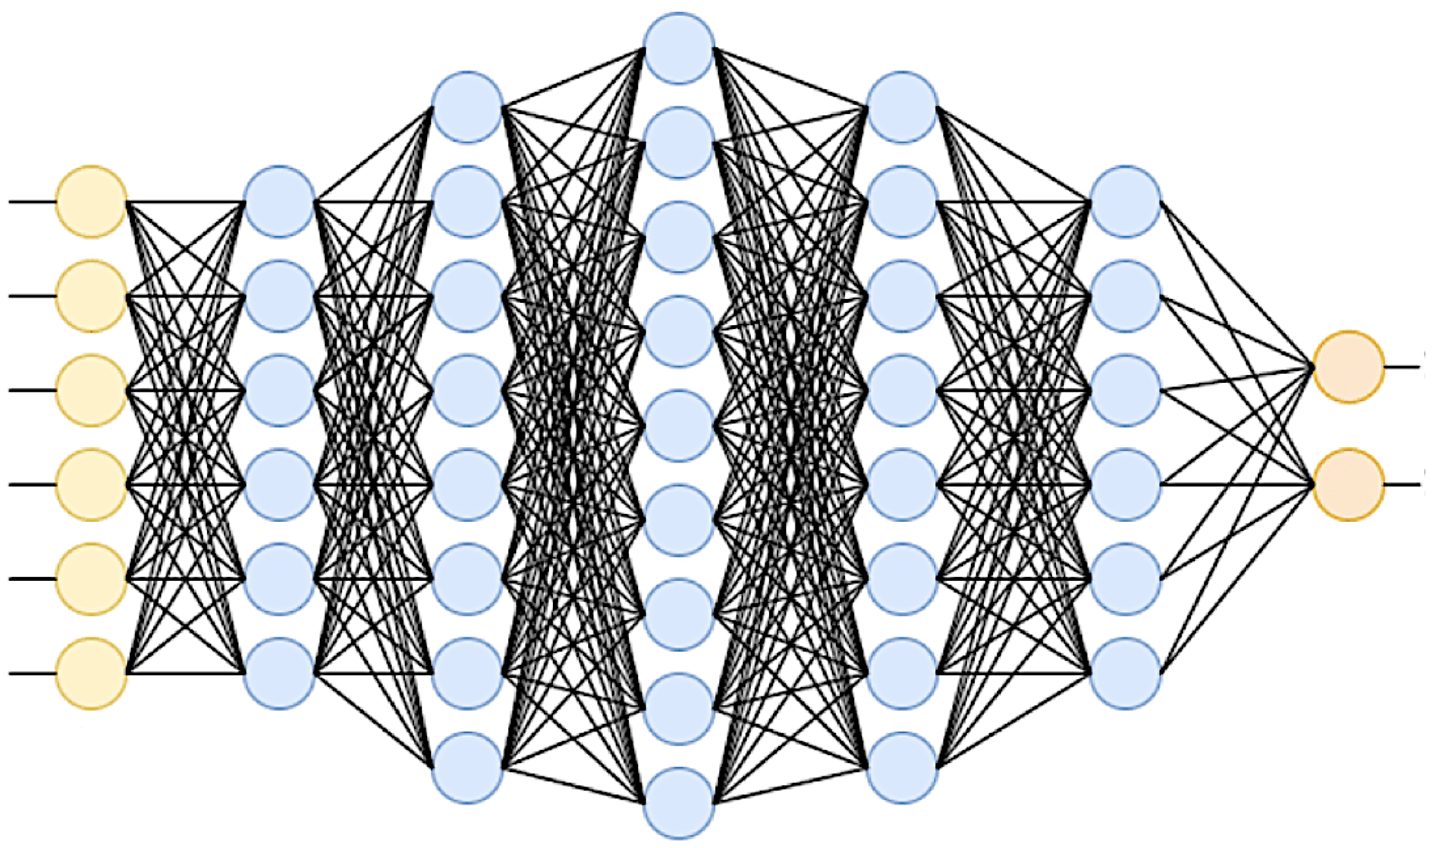
\includegraphics[keepaspectratio, scale=0.4]
 	{Figure/Deeplearning/dnn.png}
 		\caption{ディープニューラルネットワーク}
 		\label{dnn}
	\end{center}
\end{figure}
\section{グラフニューラルネットワーク}
深層学習では数値データのみでなく、画像認識や自然言語処理など様々なデータに対して目覚ましい成果を挙げている。その中で特に近年、グラフで表される構造データに対する研究が非常に盛んになっており、本研究において取り上げるグラフニューラルネットワーク(Graph Neural Network; GNN)\cite{gnnreview}もその一つである。グラフ構造データとは、オブジェクトの集合(ノード)を関係(エッジ)で結んだデータのことで、ノードのみが特徴量を持つ場合と、ノードとエッジの両方が特徴量を持つ場合がある。代表的には友人関係や論文の引用関係、化学化合物などをグラフデータとして構築することは有用であるとされており、データ間の相互関係を用いたモデリング・学習が可能であることを強みとしている。グラフの種類は大きく分けてノードの次元が同じ同種グラフと、異なる次元のデータを扱う異種グラフの2種類に分けられる。更に、エッジが方向性を持っている有向グラフと無向グラフ、データが時系列で変化する動的グラフと変化しない静的グラフに分けられる。そしてこのようなグラフデータを扱うニューラルネットをグラフニューラルネットワークという。グラフ構造や演算技術、目的とする課題によってGNNのネットワークモデルの種類は多岐にわたっており、以下では基本的なグラフでの演算や本論文に関連した幾つかの種類のモデルを取り上げる。

\subsection{メッセージパッシング}
GNNのアーキテクチャにおいて、グラフは集合$\mathcal{G} = (\mathcal{V}, \mathcal{E})$で構成されており、$\mathcal{V}$はノードの集合、$\mathcal{E}$はエッジの集合を表す。ニューラルネットワークの場合と同様にノードは特徴量を持っており、エッジも特徴量を持つことができる。図\ref{messagepass}にGNNにおける一般的な演算処理の流れ(メッセージパッシング)を示す。各ノードを$\bm{h}_i$とすると、隣接しているノードおよびその間のエッジの特徴量を集約し、ノードを更新$\bm{h}'_1$する。これによってエッジによって関連づけられたノード間で特徴量を更新していくことができる。エッジが特徴量を持つ場合は、エッジについても更新を行う。これらを数式にまとめると次のようになる。
\begin{align}
\bm{h}_{(i,j)} &= f_{\mathrm{edge}}(\bm{h}_i, \bm{h}_j, x_{(i, j)})\\
\bm{h}'_i &= f_{\mathrm{node}}(\bm{h}_i, \sum_{j\in \mathcal{N}_i}, \bm{h}_{(j, i)}, x_i)
\label{gnnm}
\end{align}
ここで、$\bm{h}_{(i,j)}$はエッジを、$x_i$はノードの特徴量を、$\mathcal{N}_i$は隣接しているノードの集合を表す。
\begin{figure}[H]
	\begin{center}
 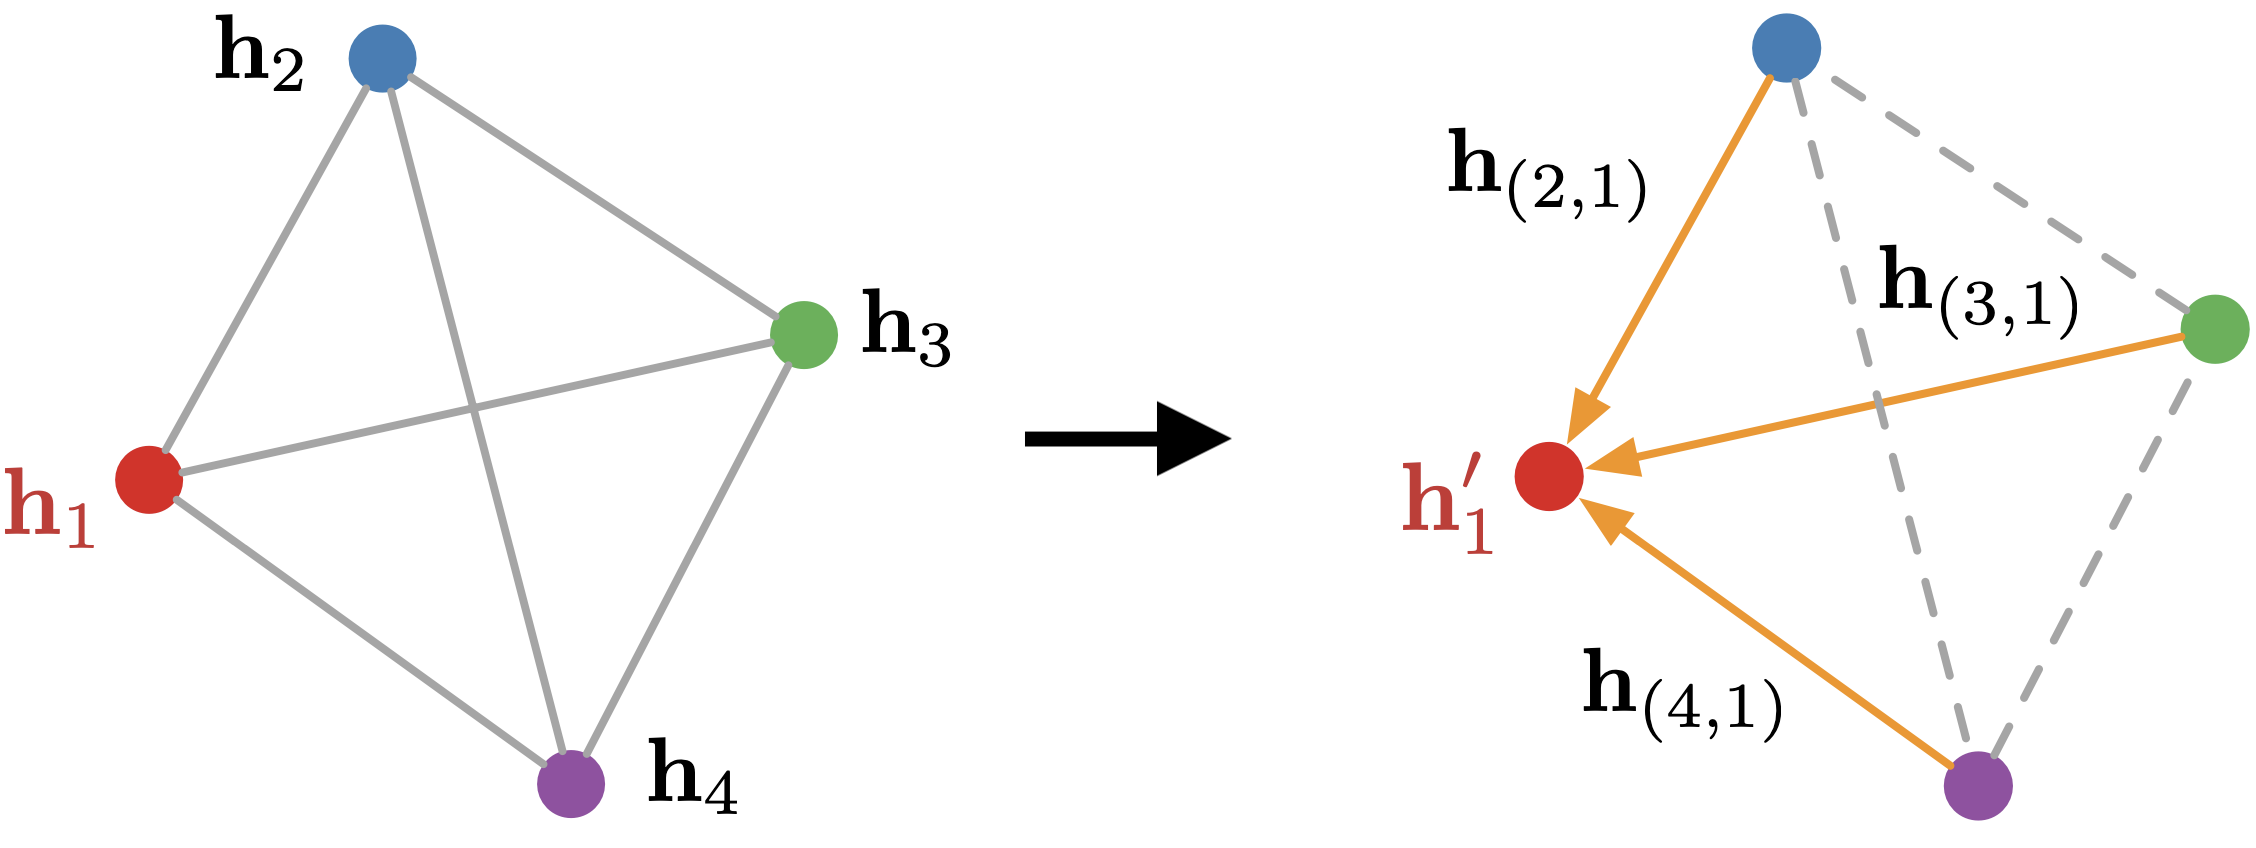
\includegraphics[keepaspectratio, scale=0.25]
 	{Figure/Deeplearning/messagepassing.png}
 		\caption{ (左) 4つのノードを持つ全結合グラフニューラルネットワーク。$h_i$はノード表現を表す。 (右) メッセージパッシングの処理。}
 		\label{messagepass}
	\end{center}
\end{figure}
\subsection{Graph Convolution Network (GCN)}
GCNとは、メッセージパッシングにおいて畳み込み(Convolution)を用いる手法である。一般的に機械学習における畳み込みは、あるフィルターを用いて対象と掛け合わせたものの和をとることで、周辺の情報を含ませることのできる処理であり、画像処理などにおいて広く用いられている。グラフの畳み込みにおいてはスペクトルによるアプローチと空間的なアプローチの2つがあり、以下ではそれぞれについて説明する。
\subsubsection{Spectral Graph Convolution}
スペクトルによる畳み込み\cite{gnnbook}は信号処理の考えに基づいたアプローチである。音声などの信号処理においては、関数をフーリエ変換によって周波数成分に変換し、ノイズ除去をして逆変換する。これをグラフデータに置き換えると、グラフラプラシアンの固有ベクトルが張る空間への変換・逆変換となる。グラフ信号を$\bm{x}$とすると、グラフフーリエ変換$\mathscr{F}(\bm{x})$、逆グラフフーリエ変換$\mathscr{F}^{-1}(\bm{x})$は次のように表される。
\begin{align}
\mathscr{F}(\bm{x}) &= \bm{U}^T\bm{x}\\
\mathscr{F}^{-1}(\bm{x}) &= \bm{U}\bm{x}
\end{align}
ここで、$\bm{U}$は正規化グラフラプラシアン$\bm{L}'$の固有ベクトル行列を表す。グラフラプラシアン$\bm{L}$は、グラフの隣接を表す隣接行列$\bm{A}$とグラフの各ノードに接続したノード数を対角成分にもつ次数行列$\bm{D}$を用いて、$\bm{L} = \bm{D}-  \bm{A}$で求められる実対称正方行列であり、正規化グラフラプラシアンは$\bm{L}' = \bm{I} - \bm{D}^{\frac{1}{2}} \bm{A} \bm{D}^{\frac{1}{2}}$とかける。\\
 これらを用いて、グラフにおけるSpectralな畳み込み演算は次のように定義される。
\begin{align}
\bm{g} \star \bm{x} &= \mathscr{F}^{-1}(\mathscr{F}(\bm{g}) \odot \mathscr{F}(\bm{x}))\\
&= \bm{U}(\bm{U}^T \bm{g} \odot \bm{U}^T \bm{x})
\end{align}
$\bm{g} \star \bm{x}$は畳み込み演算を、$\bm{U}^T \bm{g}$はスペクトルにおける畳み込みのフィルターを表す。学習により更新される集合である$\bm{g}$に焦点を当ててより単純化すると、畳み込みは次のように書くことができる。\\
\begin{align}
\bm{g} \star \bm{x} &= \bm{U} \bm{g} \bm{U}^T \bm{x}
\end{align}
 上記のように、スペクトルによる畳み込みは一度の更新の中でグラフ構造の一部が全体に影響を与えるような演算であるという特徴を持っている。さらに、行列の次元が固定されてしまうことから異なる構造のグラフ間でパラメータを共有できないことや、行列の固有値分解など計算量が多くなってしまうという問題点がある。
\subsubsection{Spatial Graph Convolution}
グラフデータにおける畳み込みは空間的なメッセージパッシングの考えに基づいており、グラフ内の1つのノードが持っている特徴量に、隣接関係にあるノードの特徴量に重みをかけたものを加えていく。これによりノード自体の特徴量に加え、隣接関係や隣接ノードの特徴量の情報などを含んだ演算を行うことができる。メッセージパッシングにおける工夫に応じて様々な畳み込みのモデルが提案されているが、以下では最も一般的なモデルであるGraphSAGE(Graph SAmple and aggreGatE)\cite{graphsage}について述べる。\\
 GraphSAGEでは、隣接から特徴量をサンプリングして集約することで自身のノードを更新する。GraphSAGEにおける畳み込み演算は式\ref{gnnm}と同様に、次の式のように表される。\\
\begin{align}
&\bm{h}_{\mathcal{N}(v)}^k \leftarrow \mathrm{AGGREGATE}_k(\{ \bm{h}_u^{k-1}, \forall u \in \mathcal{N}(v) \})\\
&\bm{h}_v^k \leftarrow \sigma (\bm{W}^k \cdot \mathrm{CONCAT}(\bm{h}_v^{k-1}, \bm{h}_{\mathcal{N}(v)}^k))\\
&  (\forall k \in \{1, ..., K\}, \forall v \in \mathcal{V}) \nonumber
\end{align}
ここで、$K$は集約における隣接の深さを、$\bm{W}^k$は重みパラメータ行列を、$\sigma$は非線形関数を表しており、1式目$\mathrm{AGGREGATE}$で集約を、2式目$\mathrm{CONCAT}$で更新を行なっている。これらの学習の処理を図\ref{sage}に示す。GraphSAGEはあらかじめサンプリングによって、隣接するノード数が異なる場合やグラフ構造が変わった場合にも畳み込み演算を行うことができ、さらに大規模なグラフ演算に対しては計算コストを改善することができる。
\begin{figure}[H]
	\begin{center}
 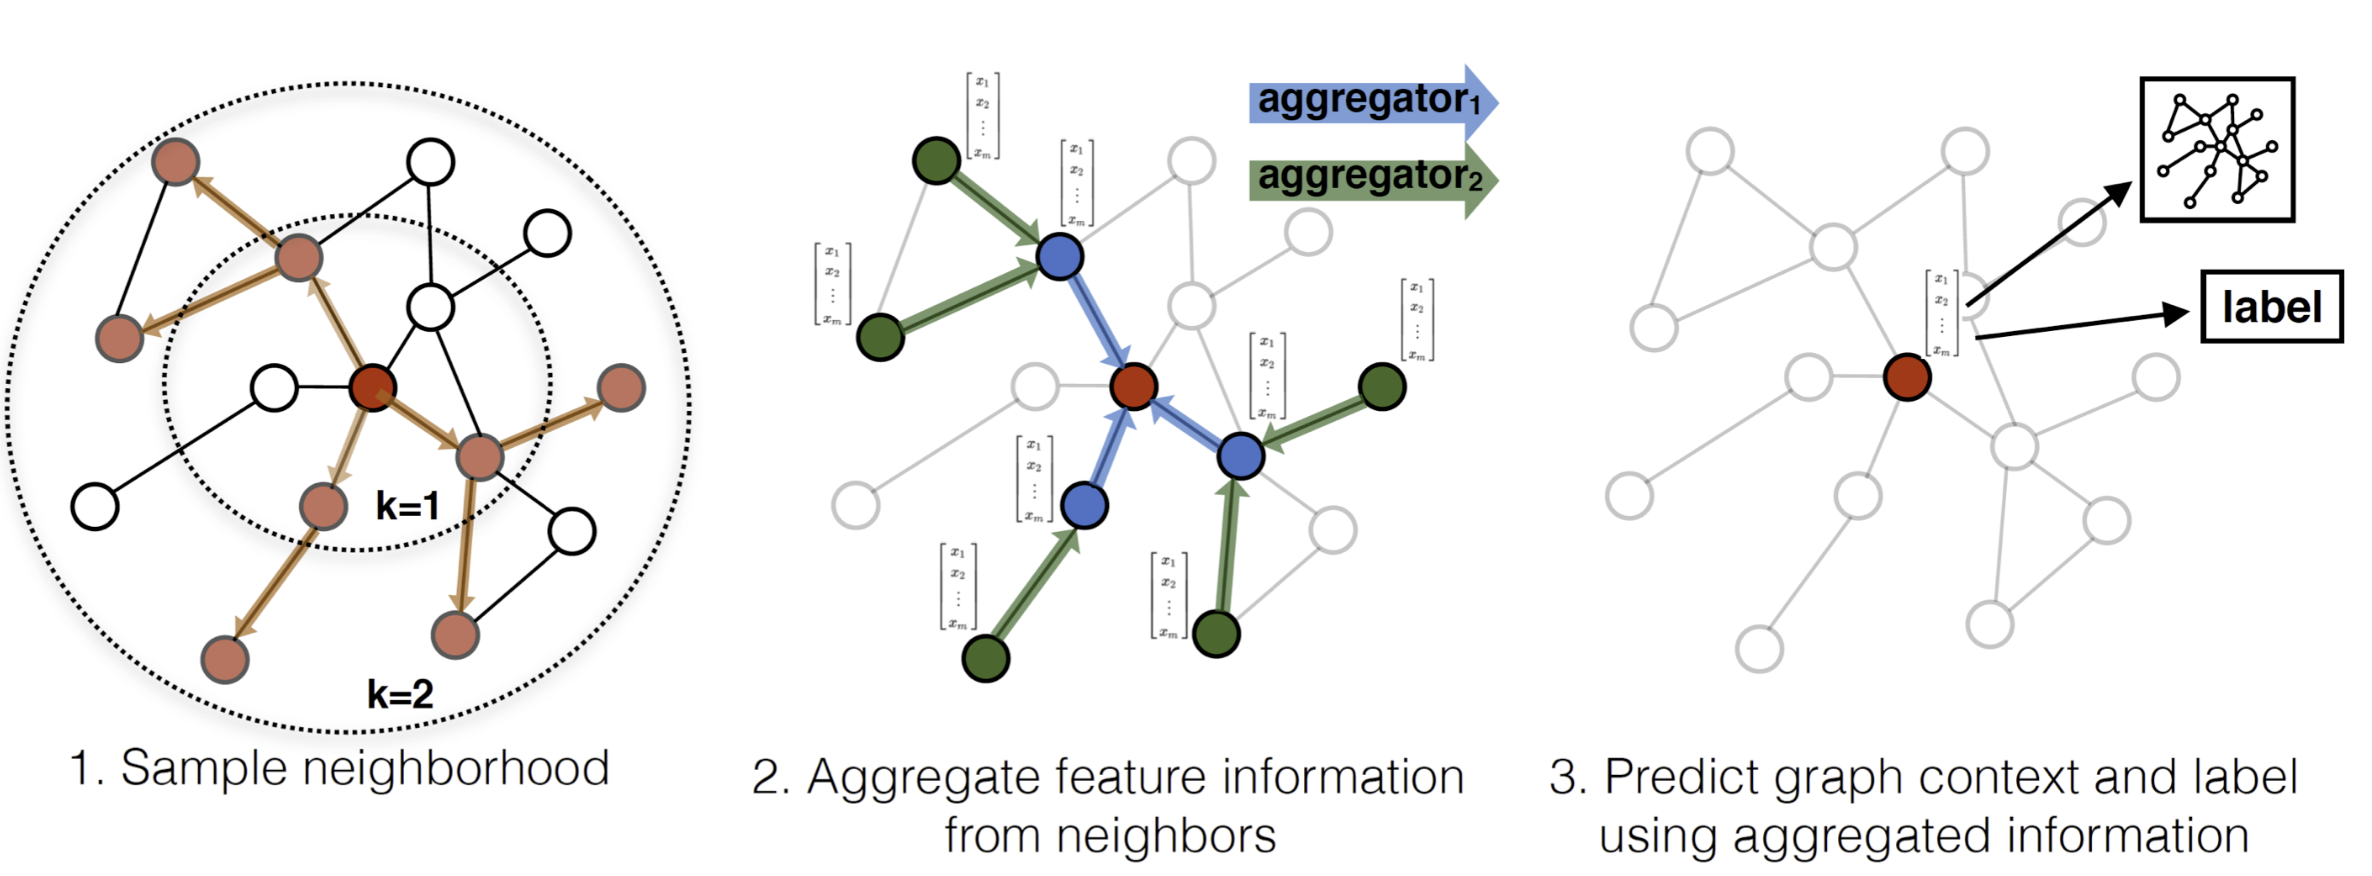
\includegraphics[keepaspectratio, scale=0.3]
 	{Figure/Deeplearning/sage.png}
 		\caption{GraphSAGEにおける処理(1. サンプリング, 2. 隣接からの集約, 3. 学習結果による推論)}
 		\label{sage}
	\end{center}
\end{figure}
\subsection{Graph Attention Network (GAT)}
\label{GATexplain}
深層学習ではAttentionという、データの中でも特に有益な場所に重み付けを行う手法があり、自然言語処理の分野などにおいてよく用いられている。Attention機構では各ノードに対して重要度を表す重みを導入し、それらを掛けた和をとることで必要な場所に注目(attention)を向けることができる。Attentionをグラフ学習に適用したものが、Graph Attention Networks (GAT) \cite{gat} である。GATでは、重みパラメータ$\bm{W}$に加えて隣接したノードの重要度を表すattention係数$\alpha_{ij}$を導入して、ノードの特徴量の更新を以下のように行う。
\begin{align}
\bm{h} = \sigma (\sum_{j \in \mathcal{N}_i} \alpha_{ij} \bm{W} \bm{h}_i )
\end{align}
ここで、$\alpha_{ij}$はattention処理$\bm{a}$を用いて、次のように表される。
\begin{align}
\alpha_{ij} &= \bm{a}(\bm{W}\bm{h}_i, \bm{W}\bm{h}_j)\\
 &= \frac{e^{\mathrm{LeakyReLU}(\bm{a}^T [ \bm{W}\bm{h}_i \parallel \bm{W}\bm{h}_j ])}}{\sum_{\mathcal{N}_i} e^{\mathrm{LeakyReLU}(\bm{a}^T [ \bm{W}\bm{h}_i \parallel  \bm{W}\bm{h}_j ])}}
\label{gatattention}
\end{align}
 GATではattention処理に1層のニューラルネットワークを用いており、$\bm{a}$として学習の重みベクトルを用いている。式\ref{gatattention}においては全ノード間で正規化して確率値を出力するためのsoftmax関数の適用と、活性化関数 (Leaky ReLU) の適用を行っている。($\parallel$はテンソルのconcatenateを表す。)これらの演算処理のイメージを図\ref{gatt}に示す。GATは、隣接に任意の重みを割り当てることから次数の異なるノードにも適応可能であり、未知のグラフ構造にも一般化することができる。
\begin{figure}[H]
	\begin{center}
 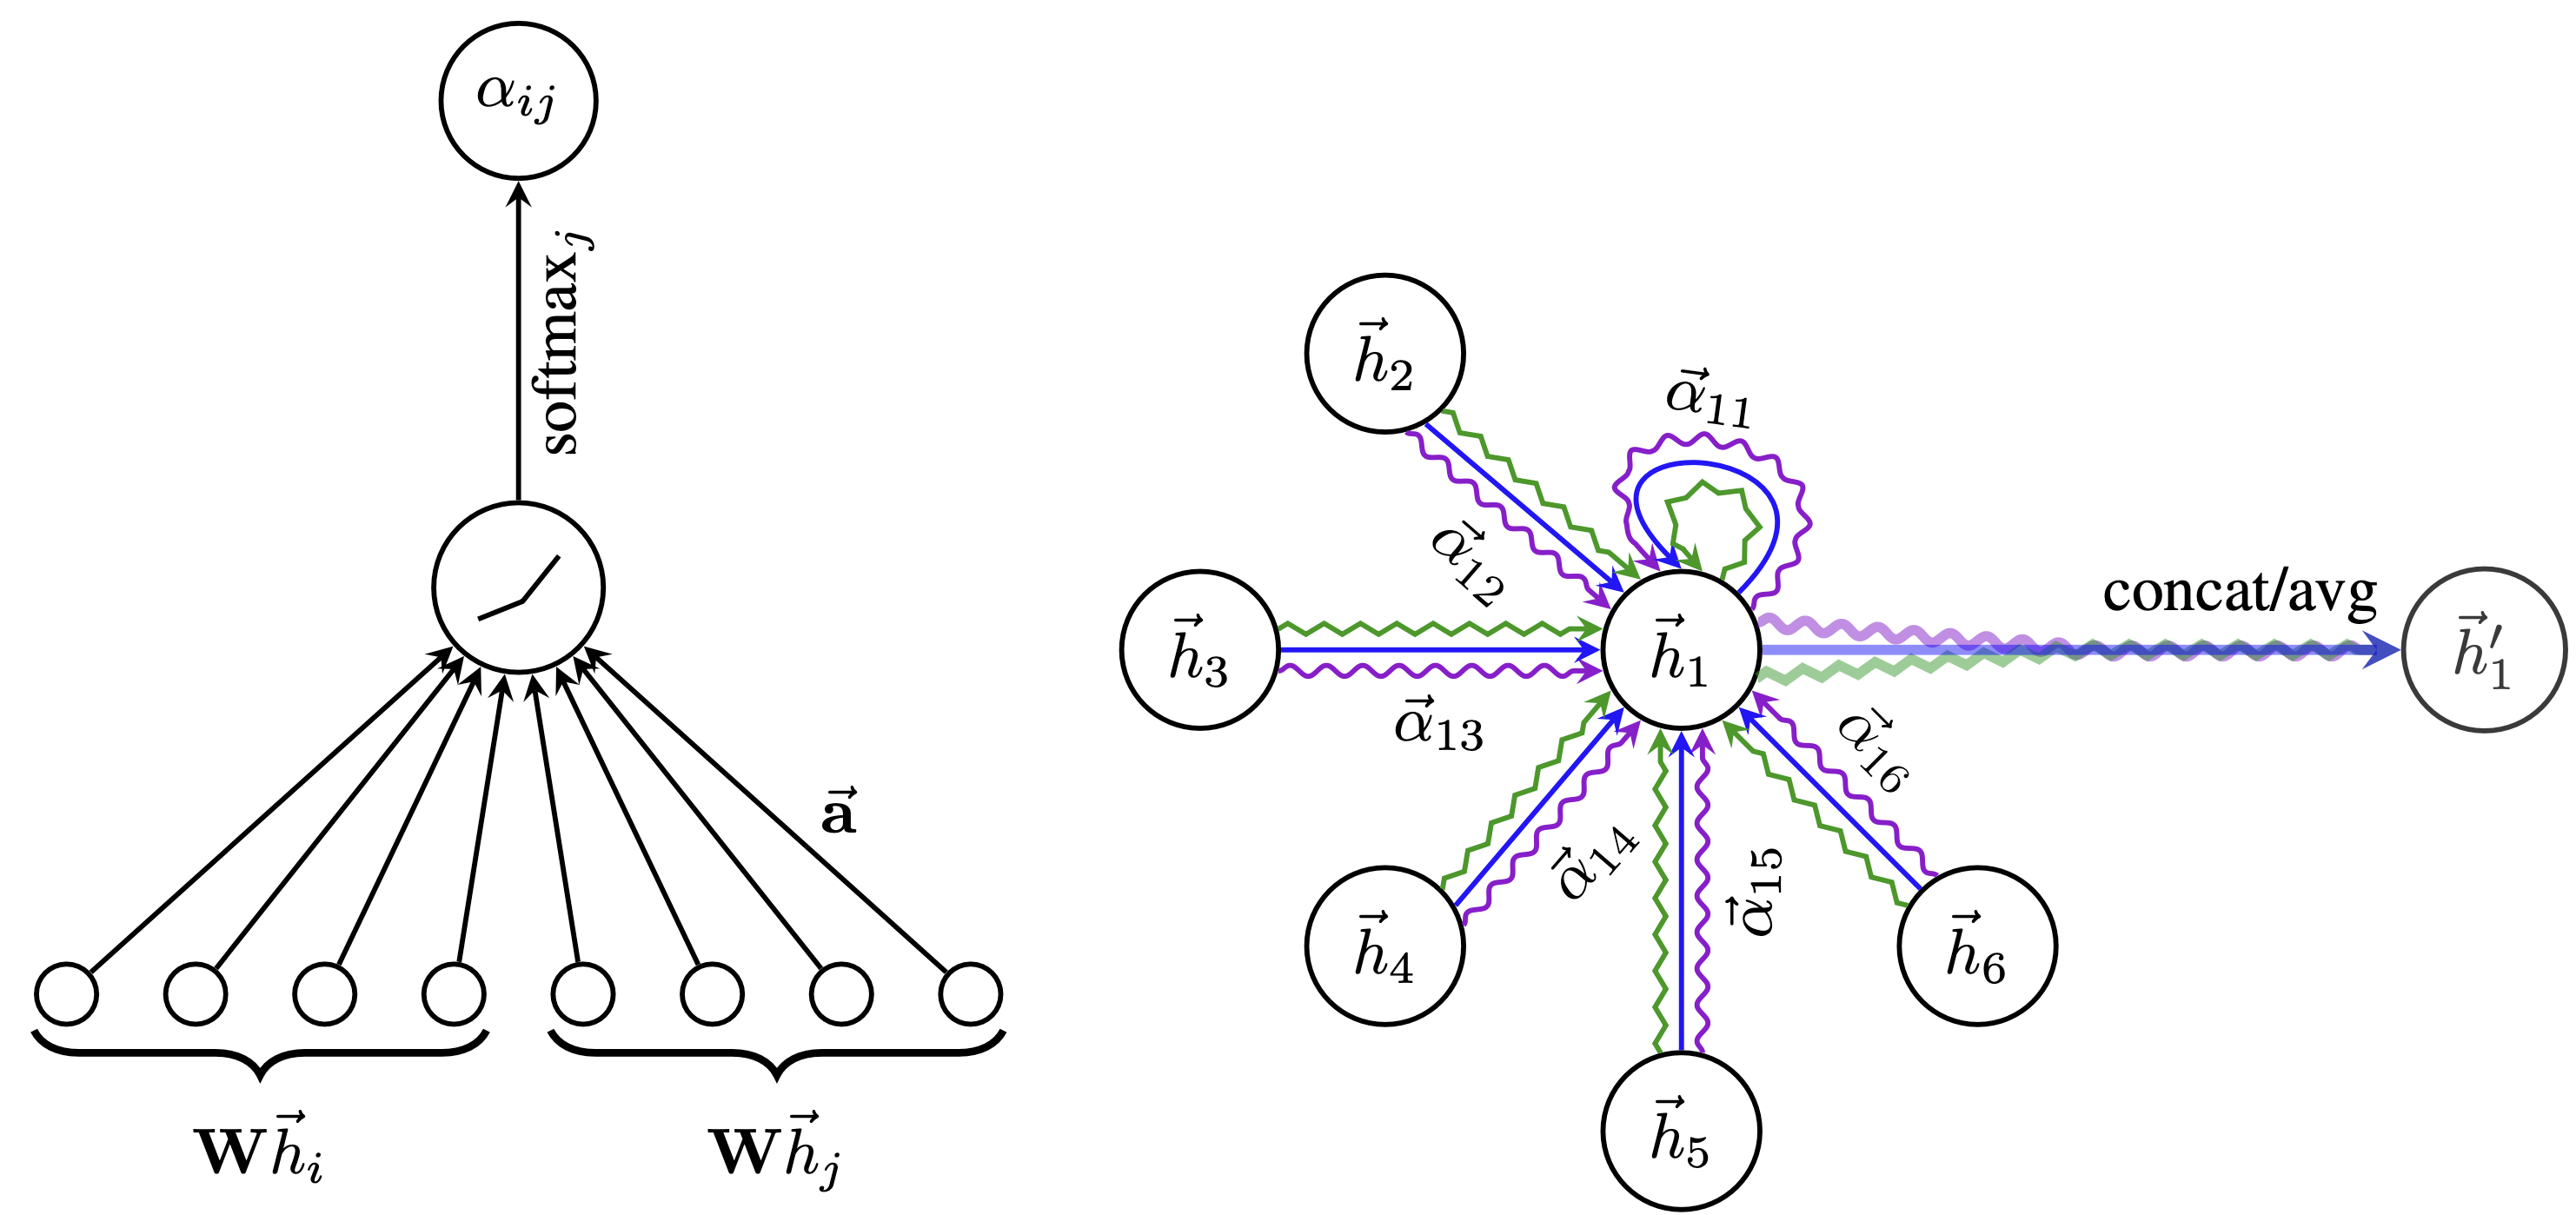
\includegraphics[keepaspectratio, scale=0.25]
 	{Figure/Deeplearning/gat.png}
 		\caption{ (左) 重みベクトル$\bm{a}$を用いたAttention処理。 (右) 1つのノード$\bm{h}_1$に対する隣接ノード$\bm{h}_{\neq 1}$のAttentionと、ノード特徴量の更新$\bm{h'}_1$}
		\label{gatt}
	\end{center}
\end{figure}